\begin{table}[t]
\centering
\caption{Feature comparison of physics-based differentiable radar renderers. Signal: ADC\,=\,raw FMCW, CIR\,=\,channel impulse response, IF\,=\,intermediate-frequency phasors. Multi-b.\,=\,multi-bounce; Diffr.\,=\,edge diffraction; Polar.\,=\,polarization; Geom.\,=\,differentiable geometry; Norm.\,=\,differentiable normals; Mat.\,=\,physics material model; Per-vtx\,=\,per-vertex materials; Bound.\,$\nabla$\,=\,boundary gradients; Real\,=\,validated on real data. Checkmarks denote supported pipeline capabilities; see Sec.~\ref{sec:supp_training} in the supplement for which parameters are active in our experiments.}
\label{tab:polarization_comparison}
\small
\setlength{\tabcolsep}{3pt}
\renewcommand{\arraystretch}{1.1}
\resizebox{\linewidth}{!}{
\begin{tabular}{|l|c|c|c|c|c|c|c|c|c|c|c|c|c|c|}
\hline
\rowcolor{mediumgray}
\textbf{Method} &
\textbf{Open} &
\textbf{Repr.} &
\textbf{Signal} &
\textbf{Multi-b.} &
\textbf{Diffr.} &
\textbf{Polar.} &
\textbf{Geom.} &
\textbf{Norm.} &
\textbf{Mat.} &
\textbf{Pose} &
\textbf{Beam} &
\textbf{Per-vtx} &
\textbf{Bound. $\nabla$} &
\textbf{Real} \\
\hline
\cellcolor{lightergray}Sionna RT~\cite{sionna} &
\cellcolor{lightgreen}$\checkmark$ &
\cellcolor{lightgreen}Mesh &
\cellcolor{lightyellow}CIR &
\cellcolor{lightgreen}$\checkmark$ &
\cellcolor{lightgreen}$\checkmark$ &
\cellcolor{lightgreen}$\checkmark$ &
\cellcolor{lightred}-- &
\cellcolor{lightred}-- &
\cellcolor{lightyellow}No BRDF &
\cellcolor{lightgreen}$\checkmark$ &
\cellcolor{lightred}-- &
\cellcolor{lightred}-- &
\cellcolor{lightred}-- &
\cellcolor{lightred}-- \\
\hline
\cellcolor{lightergray}SFCW Inv.~\cite{hofmann2025inverse} &
\cellcolor{lightgreen}$\checkmark$ &
\cellcolor{lightgreen}Mesh &
\cellcolor{lightyellow}IF &
\cellcolor{lightred}-- &
\cellcolor{lightred}-- &
\cellcolor{lightgreen}$\checkmark$ &
\cellcolor{lightred}-- &
\cellcolor{lightyellow}Shading &
\cellcolor{lightgreen}$\checkmark$ &
\cellcolor{lightyellow}Pos. &
\cellcolor{lightred}-- &
\cellcolor{lightgreen}$\checkmark$ &
\cellcolor{lightred}-- &
\cellcolor{lightgreen}$\checkmark$ \\
\hline
\cellcolor{lightergray}InverTwin~\cite{chen2025invertwin} &
\cellcolor{lightred}-- &
\cellcolor{lightgreen}Mesh &
\cellcolor{lightyellow}CIR &
\cellcolor{lightgreen}$\checkmark$ &
\cellcolor{lightgreen}$\checkmark$ &
\cellcolor{lightred}-- &
\cellcolor{lightgreen}$\checkmark$ &
\cellcolor{lightred}-- &
\cellcolor{lightyellow}No BRDF &
\cellcolor{lightgreen}$\checkmark$ &
\cellcolor{lightred}-- &
\cellcolor{lightred}-- &
\cellcolor{lightgreen}$\checkmark$ &
\cellcolor{lightgreen}$\checkmark$ \\
\hline
\cellcolor{lightergray}mmIR (Ours) &
\cellcolor{lightgreen}$\checkmark$ &
\cellcolor{lightgreen}Mesh &
\cellcolor{lightgreen}ADC &
\cellcolor{lightgreen}$\checkmark$ &
\cellcolor{lightgreen}$\checkmark$ &
\cellcolor{lightgreen}$\checkmark$ &
\cellcolor{lightgreen}$\checkmark$ &
\cellcolor{lightgreen}$\checkmark$ &
\cellcolor{lightgreen}$\checkmark$ &
\cellcolor{lightgreen}$\checkmark$ &
\cellcolor{lightgreen}$\checkmark$ &
\cellcolor{lightgreen}$\checkmark$ &
\cellcolor{lightgreen}$\checkmark$ &
\cellcolor{lightgreen}$\checkmark$ \\
\hline
\end{tabular}
}
\end{table}

\section{Related Works}

\textbf{Differentiable rendering beyond optics.}
Differentiable rendering couples explicit scene parameterizations with gradient-based optimization to recover geometry, materials, and sensor parameters~\cite{veach1995optimally, veach1998robust, ramamoorthi2007first, gargallo2007minimizing}. Core advances include analytic inverse rendering and MC estimator reparameterizations~\cite{li2018differentiable,loubet2019reparameterizing, bangaru2020unbiased}, as well as practical path tracing systems and neural/hybrid representations~\cite{mildenhall2021nerf, 10.1145/3550469.3555397, zhang2022iron, 10.1145/3355089.3356498, jakob2022dr, bangaru2023slang}. These methods operate almost exclusively in the optical regime. In RF, Sionna RT~\cite{sionna} propagates gradients through field coefficients and CIR computation but not through path topology: its path solver runs under gradient suspension and subsequently detaches all path geometry, so vertex positions and surface normals receive no gradients, restricting inverse rendering to quantities that enter only the CIR computation (antenna patterns, scattering coefficients, TX/RX positions). It also does not model wideband FMCW signals; Hofmann et al.~\cite{hofmann2025inverse} estimate SFCW materials but require known geometry, model only single-bounce propagation, and treat visibility as non-differentiable; and InverTwin~\cite{chen2025invertwin} addresses multipath gradient pathologies via path-space differentiation but substitutes a Gaussian kernel surrogate for radar range processing and validates on synthetic data only. mmIR bridges this gap with end-to-end AD through ray tracing itself, enabling gradients to flow through all bounces back to geometry, materials, and sensor parameters directly from raw frequency-space FMCW ADC (Table~\ref{tab:polarization_comparison}).

\begin{figure}[t]
  \centering
  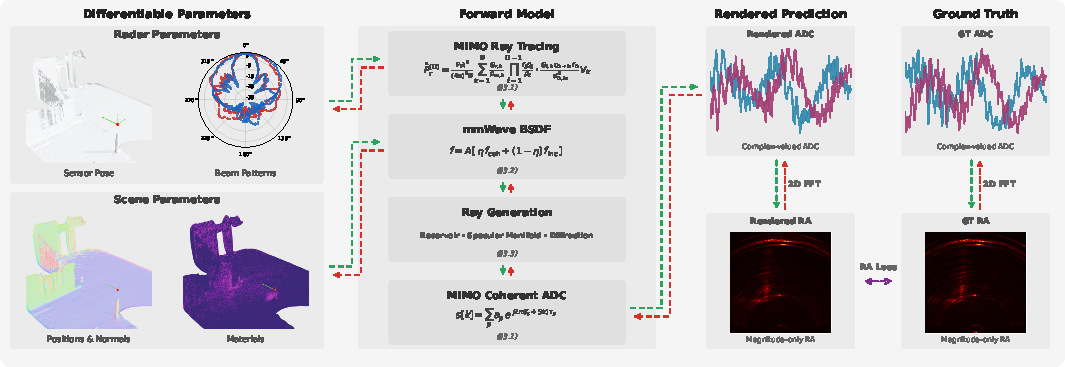
\includegraphics[width=\linewidth]{figs/pipeline/pipeline_v3.pdf}
  \caption{Overview of the mmIR pipeline. Given a LiDAR-derived mesh and initial sensor parameters, the differentiable forward model traces phase-coherent MIMO paths via multiple importance sampling over reflection and diffraction for all TX--RX pairs, then synthesizes raw FMCW ADC. End-to-end automatic differentiation through the full path (ray tracing $\to$ BSDF $\to$ phasor accumulation $\to$ ADC) enables joint optimization of per-vertex materials, geometry, normals, and 6-DoF radar pose from a range--azimuth reconstruction loss.}
  \label{fig:system}
\end{figure}

\textbf{Ray tracing for FMCW signal modeling.}
Radar simulation typically employs shooting-and-bouncing rays (SBR) to scale beyond full-wave solvers, producing path geometry and attenuation for large scenes and MIMO arrays~\cite{dudek2010millimeter}. Recent computational RF imaging further demonstrates multi-bounce physics for reconstruction on real mmWave hardware~\cite{dodds2025mito}. However, these pipelines are forward-only: scene and sensor parameters are fixed, precluding calibration against real captures. mmIR makes SBR-style FMCW rendering fully differentiable, exposing gradients w.r.t.\ mesh geometry, per-vertex materials, radar pose, and antenna patterns to close the sim-to-real gap.

\textbf{Neural and Gaussian methods for radar data synthesis.}
Neural fields have been adapted to radar across modalities: SAR/ISAR shape reconstruction~\cite{lei2024sar,deng2024isar}, FMCW occupancy and Doppler recovery~\cite{takawale2025spinr,huang2024dart}, frequency-space response synthesis~\cite{10.1145/3641519.3657510,zhang2025rf4d}, and multi-modal fusion with RGB/LiDAR~\cite{rafidashti2025neuradar,lu2024newrf}. RadarSplat~\cite{kung2025radarsplat} provides a Gaussian splatting~\cite{3dgs} alternative for range--azimuth rendering. These methods learn opaque, sensor-specific representations: DART~\cite{huang2024dart} discards phase entirely (magnitude-only range--Doppler supervision), none expose physically interpretable material parameters, and none model multi-bounce propagation, polarization, or diffraction. Moreover, methods that render post-processed images directly must learn to reproduce FFT point-spread artifacts (sidelobes, windowing); by rendering raw ADC, mmIR applies identical FFT processing to both rendered and measured data, cleanly decoupling scene physics from signal processing. mmIR maintains an explicit mesh with per-vertex ITU materials and polarization-aware BSDFs, enabling joint scene--sensor calibration and re-rendering from arbitrary virtual apertures for 3D imaging.

% \section{Related Works}

% \subsection{Differentiable Rendering}

% Classical differentiable rendering couples explicit or implicit 3D scene representations with gradient-based optimization to recover geometry, materials, and camera parameters from images~\cite{veach1995optimally, veach1998robust, ramamoorthi2007first, gargallo2007minimizing}. Early work focused on analytic inverse rendering and reparameterizations of Monte Carlo estimators~\cite{li2018differentiable,loubet2019reparameterizing, bangaru2020unbiased}, while more recent methods combine NeRF-style volumetric representations with differentiable path tracing~\cite{mildenhall2021nerf, 10.1145/3550469.3555397, zhang2022iron} and practical systems such as Mitsuba 2~\cite{10.1145/3355089.3356498}, Dr.Jit~\cite{jakob2022dr}, and Slang.d~\cite{bangaru2023slang} for general-purpose inverse rendering. These approaches operate almost exclusively in the optical regime and assume narrowband sensors with simple projective geometry. Sionna RT tackles this by extending differentiable ray tracing to the RF domain for wireless communications, exposing gradients with respect to antenna patterns, materials, and deployment parameters~\cite{sionna}, but it targets link-level channel metrics rather than high-resolution 3D imaging and does not model FMCW-specific signal generation or raw ADC samples. Hofmann et al.  introduce an SFCW radar inverse renderer that estimates material parameters from near-field measurements given known geometry~\cite{hofmann2025inverse}, and InverTwin proposes a differentiable RF digital twin that addresses gradient pathologies from multipath and path creation/destruction at the level of channel responses~\cite{chen2025invertwin}. mmIR is complementary to these efforts. We specialize differentiable rendering to wideband FMCW radar and operate directly in frequency-space ADC coordinates, with a multi-bounce, polarization-aware, diffraction-enabled forward model. Table~\ref{tab:polarization_comparison} compares and evaluates our proposed method against three other radar inverse renderers.

% % Need better version of this: Unlike RF digital twins that optimize path-wise channel coefficients, mmIR jointly optimizes b LiDAR-registered mesh geometry, per-vertex materials, radar pose, and per-antenna patterns from real FMCW captures and then re-uses the optimized scene as a generator for wide virtual apertures.

% \subsection{Ray Tracing for Radar Data Synthesis}

% Physics-based radar simulation has a long history in microwave imaging and remote sensing. Full-wave solvers that directly discretize Maxwell’s equations offer high accuracy but are too expensive for large scenes or repeated optimization. To improve scalability, many works adopt high-frequency approximations such as shooting-and-bouncing rays (SBR), modeling propagation via geometric optics plus heuristic diffraction terms. Recent simulators for automotive radar build on these ideas to support large MIMO arrays and digital-twin environments, combining CAD models with ray tracing and simplified material models for specular and diffuse scattering. For FMCW radar, Dudek et al.\ derive a frequency-domain signal model that connects transmitted chirps, propagation paths, and sampled baseband signals, providing a bridge between ray-tracing outputs and the ADC domain used in hardware~\cite{dudek2010millimeter}. In parallel, computational RF imaging systems such as MITO demonstrate that carefully designed multi-bounce imaging setups can recover geometry through occluders using optimization on real mmWave hardware~\cite{dodds2025mito}. These frameworks are typically used in a purely forward or task-specific manner: geometry and materials are fixed, and simulators generate synthetic data without gradient feedback, or reconstruction pipelines are tied to a particular sensor. mmIR builds directly on SBR-style multi-bounce ray tracing and FMCW signal modeling, but turns them into a general-purpose differentiable inverse renderer. We integrate polarization-aware BRDFs and edge diffraction into an FMCW frequency-space forward model and expose gradients with respect to mesh geometry, per-vertex materials, vertex normals, radar pose, and per-antenna patterns, allowing us to optimize and fit raw frequency-space ADC radar data to real captures, and then re-render as wide synthetic arrays for 3D mmWave reconstruction.

% \subsection{Neural Methods for Radar Data Synthesis}

% Neural radiance fields and related implicit representations have transformed view synthesis and 3D reconstruction in the optical domain~\cite{mildenhall2021nerf,kerbl20233d}, and extensions to LiDAR and multi-sensor fusion have shown benefits from incorporating explicit range measurements. A growing body of work adapts these ideas to radar. SAR-NeRF and ISAR-NeRF formulate NeRF-style inverse problems for SAR and ISAR, respectively, reconstructing voxel grids or target shapes from radar images using differentiable SAR imaging equations~\cite{lei2024sar,deng2024isar}. SpINR couple an implicit neural volume with a differentiable frequency-domain FMCW forward model to recover dense occupancy from raw radar data~\cite{takawale2025spinr}. For automotive-style FMCW radar, DART learns an implicit Doppler tomography representation from range–Doppler data for novel-view synthesis and multipath analysis~\cite{huang2024dart}. Radar Fields synthesizes raw radar data directly in frequency space, learning a neural field that map 3D coordinates and view direction to complex FMCW responses and occupancy for scanning trajectories~\cite{10.1145/3641519.3657510}. RF4D extends neural fields to dynamic outdoor driving scenes by treating time as an additional dimension~\cite{zhang2025rf4d}. NeuRadar and NeWRF train NeRF-style models on sparse automotive radar point clouds jointly with RGB/LiDAR to enable multi-modal novel view synthesis and radar simulation in adverse weather~\cite{rafidashti2025neuradar,lu2024newrf}. Rather than learning a purely neural volume, we start from a LiDAR-registered mesh with physically interpretable per-vertex materials and normals, and fit this scene directly to raw frequency-domain FMCW data consistent with radar physics. This allows us to jointly calibrate scene and sensor parameters, maintain compatibility with graphics BRDF models, and then render synthetic wide-aperture arrays for 3D reconstruction, instead of only learning a forward neural mapper from radar signals to occupancy or images.

% \subsection{Gaussian Splatting for Radar Data Synthesis}

% Gaussian splatting offers an explicit, real-time alternative to NeRF by representing scenes as a set of anisotropic 3D Gaussians optimized for view synthesis~\cite{3dgs}. In the optical domain, Gaussian splatting achieves high-fidelity, real-time rendering on large-scale datasets and has been extended to panoramic cameras and RGB-D streams. These methods typically assume photometric radiance accumulation and camera-based sensor models. Recent work adapts Gaussian splatting to radar imaging. RadarSplat~\cite{kung2025radarsplat} introduces a Gaussian representation tailored to FMCW radar, attaching complex-valued scattering amplitudes and radar-specific attributes to each Gaussian and rendering frequency-space or range–azimuth images from scanning trajectories using a radar equation–based forward model. mmIR differs from radar Gaussian splatting in both representation and goal. We do not learn Gaussian primitives; instead, we maintain an explicit mesh-based scene with polarization-aware BRDFs and per-antenna gain models, and treat radar synthesis as differentiable FMCW rendering. This lets us directly optimize geometry, materials, and sensor parameters against real frequency-domain data and then re-render from arbitrary virtual apertures, while remaining tightly anchored to the underlying radar physics.

